\section{Basics for Group and Representation Theory}

This section gives the basic definitions about groups and representations necessary to understand this work.
We refer to the literature for a more detailed introduction \parencite{artin2011algebra,GroupRepRef}.
\label{sec:intro_to_groups}
\subsection{Groups}

A \textit{group} $(G,\cdot)$ is a set $G$ together with a function $\cdot:G\times G\to G, (g,h)\mapsto g\cdot h$ called group \emph{operation} satisfying \begin{enumerate} \item (Associativity): $g\cdot(h\cdot i)=(g\cdot h)\cdot i$ for all $g,h,i\in G$ \item (Existence of a neutral element): There is a $e\in G$ such that: $e\cdot g=g\cdot e= g$ for all $g\in G$ \item (Existence of an inverse): For all $g\in G$, there is a $g^{-1}$ such that $e=g^{-1}\cdot g=g\cdot g^{-1}$ \end{enumerate} If in addition, $G$ satisfies \begin{enumerate}[resume] \item (Commutativity): $g\cdot h=h\cdot g$ for all $g,h\in G$ \end{enumerate} $G$ is called \emph{Abelian}.
We simply write $g_1g_2$ for $g_1\cdot g_2$ if it is clear from the context.

If $\rho:G\to G'$ is a map between two groups, it is called a \emph{group homomorphism} if $\rho(g\cdot g')=\rho(g)\cdot\rho(g')$.
That is, the map preserves the action of the group.
A \emph{group isomorphism} is a homomorphism that is bijective.
In the later case, $G$ and $G'$ are called \text{isomorphic} and we write $G\cong G'$.

\textbf{The Euclidean group}

In the context of this work, the most important example of a group is the \emph{Euclidean group} $E(n)$ consisting of all \emph{isometries}, i.e. the set of all functions $T:\R^n\to\R^n$ such that \begin{align*} \|T(\mathbf{x})-T(\mathbf{x}')\|=\|\mathbf{x}-\mathbf{x}'\|,\quad\text{for all }\mathbf{x},\mathbf{x}'\in\R^n \end{align*} Defining the group operation as the composition of two isometries by $T_1\cdot T_2:=T_1\circ T_2$, we can identify $E(n)$ as a group.

\textbf{Subgroups}

A \textit{subgroup} $H$ of a group $(G,\cdot)$ is a subset $H\subset G$ which is closed under the action of the original group.
I.e. a set $\hrp\subset \grp$ is a subgroup of $(\grp, \cdot)$ if $h_1 \cdot h_2\in\hrp$ for all $h_1, h_1 \in \hrp$ and $h^{-1}\in H$ for all $h\in H$.
A subgroup is typically denoted by $\hrp < \grp$.

We can identify all intuitive geometric transformations on $\R^n$ as subgroups of $E(n)$: \begin{enumerate} \item \textbf{Translation:} For any vector $\mathbf{x}\in\R^n$, a translation by $\mathbf{x}$ is given by the map $t_\mathbf{x}:\R^n\to\R^n,\mathbf{x}'\mapsto \mathbf{x}+\mathbf{x}'$.
	      The group of all translations is denoted by $T(n)$ .
	\item \textbf{Rotoreflection:}
	      The orthogonal group $O(n)=\{Q\in\R^{n\times n}| QQ^T=I\}$ describes all reflections and subsequent rotations.
	\item \textbf{Rotation:}
	      The special orthogonal group $SO(n)=\{R\in O(n)| \det R=1\}$ describes all rotations in $\R^n$.
\end{enumerate}

\textbf{Normal subgroups}

A \textit{normal subgroup} of a group is a subgroup which is closed under conjugation of the group.
That is, $N$ is a normal subgroup of $\grp$ if it is a subgroup of $\grp$ and \begin{equation*} gng\inv \in N \; \quad\text{for all }\; n \in N, g \in \grp \end{equation*} Typically a normal subgroup is denoted $N \triangleleft \grp$.
The most important example for this work is $T(n)\triangleleft E(n)$.

\newpage
\textbf{Semidirect product groups}
\hypertarget{def:semidicrectproduct}{}

A group $G$ is a \textit{semidirect product} of a subgroup $\hrp<\grp$ and a normal subgroup $N\triangleleft\grp$ if it holds that for all $g\in G$, there are unique $n\in N,h\in H$ such that $g=nh$.
There are a number of equivalent conditions, but not needed for this exposition.
The semidirect product of two groups is denoted by \begin{equation*} \grp = N \rtimes \hrp \end{equation*} Most importantly, we can identify $E(n)=T(n)\rtimes O(n)$ as the semidirect product of $T(n)$ and $O(n)$.
\subsection{Representations of Groups}
Group representations are a powerful tool to describe the algebraic properties of geometric transformations: \hypertarget{def:representation}{} Let $V$ be a vector space and $\f{GL}(V)$ be the \textbf{general linear group}, i.e. the group of all linear, invertible transformations on $V$ with the composition $f\cdot g=f\circ g$ as group operation.
Then a \textbf{representation} of a group $H$ is a group homomorphism $\rho:\hrp\to \f{GL}(V)$.
For $V=\R^d$, this is the same as saying a group representation is a map $\rho: \hrp \to \R^{d\times d}$ such that \begin{align*} \rho(h_1\cdot h_2)=\rho(h_1) \rho(h_2) \end{align*} where the right hand side is typical matrix multiplication.

The simplest group representation is the \hypertarget{trivialrep}{\textit{trivial representation}} $\rho_{triv}$ which maps all elements of the group to the identity, \begin{align} \rho_{triv}(h) =\mathbf{1}_{d} \quad\text{for all }h\in H \end{align} 

\textbf{Orthogonal and unitary groups} 

An \hypertarget{def:orthogonal_representation}{\textit{orthogonal representation}} is a representation $\rho:H\to\f{GL}(\R^d)$ such that $\rho(h)\in O(d)$ for all $h\in H$.
For \textit{compact groups} $H$, every representation is equivalent to an orthogonal representation \parencite[Theorem II.1.7]{GroupRepRef}.
This is useful as the identity $\rho(h)^T = \rho(h)\inv$ often makes calculations significantly easier.
Since in this work we focus on subgroups $H\subset O(d)$ which are all compact, it is not a restriction to assume that.

\textbf{Direct sums}

Given two representations, $\rho_1: \hrp \to \f{GL}(\R^n)$ and $\rho_2: \hrp \to \f{GL}(\R^m)$ , we can combine them together to give their \textit{direct sum}, $\rho_1 \oplus \rho_2: H\to \f{GL}(\R^{n+m})$, defined by \begin{equation} (\rho_1 \oplus \rho_2)(h) = \begin{bmatrix} \rho_1(h) & 0 \\ 0 & \rho_2(h) \end{bmatrix} \end{equation} i.e the block diagonal matrix comprised of the two representations.
This sum generalises to an arbitrary number of representations.

\hypertarget{def:tensor_product}{\textbf{Tensor products}}

Let $V_1,V_2$ be two vector spaces and $V_1\otimes V_2$ their tensor product.
Given two representations, $\rho_1: \hrp \to \f{GL}(V_1)$ and $\rho_2: \hrp \to \f{GL}(V_2)$, we can take the tensor product representation $\rho_1 \otimes \rho_2: \hrp \to \f{GL}(V_1 \otimes V_2)$ defined by the condition that \begin{align} [\rho_1 \otimes \rho_2](h)(v_1 \otimes v_2) = (\rho_1(h)v_1) \otimes (\rho_2(h)v_2) \end{align} for all $v_1\in V_1$, $v_2\in V_2$, $h \in \hrp$.

To make this concrete for \cref{prop:SteerCNP}, we have $V_1,V_2=\R^d$ and the tensor product becomes $V_1\otimes V_2=\R^{d\times d}$ with $v_1\otimes v_2=v_1v_2^T$ the outer product for all $v_1,v_2\in\R^d$.
Setting $\rho=\rho_1=\rho_2$, the tensor product representation $\rho\otimes\rho$ becomes \begin{align} [\rho\otimes\rho](h)(v_1\otimes v_2)=(\rho(h)v_1)(\rho(h)v_2)^T =\rho(h)v_1v_2^T\rho(h)^T \end{align} Therefore, $\rho_{\Sigma}$ as defined in \cref{eq:tensor_product_representation_sigma} is the tensor product $\rho\otimes\rho$.
We can return such representations to the more usual matrix-acting-on-vector format by vectorising these expressions.
Using the identity $\f{vec}(ABC) = [C^T \otimes_{kron} A] \f{vec}(B)$, with $\otimes_{kron}$ being the usual Kronecker product and $\f{vec}(A)$ being the column-wise vectorisation of $A$ we get \begin{align} \f{vec}(\rho(h) A \rho(h)^T) = [\rho(h) \otimes_{kron} \rho(h)] \f{vec}(A) \end{align} 

\section{Proofs} \subsection{Proof of \cref{prop:inv_dist_leads_to_equiv} } \label{proof:invprior} \begin{proof} Let us be given a distribution $P$ over functions $\mathcal{F}_\rho$ and $F\sim P$.
	Define $g.P$ to be the distribution of $g.F$.
	For any $\mathbf{x}_1,\dots,\mathbf{x}_k\in\R^n$ let $\mathbf{x}_{1:k}$ denote the concatenation $(\mathbf{x}_1,\dots,\mathbf{x}_k)$ of these vectors and let $g\mathbf{x}_{1:k}$ be $(g\mathbf{x}_1,\dots,g\mathbf{x}_k)$.
	For any such $\mathbf{x}_{1:k}$, let $\psi_{\mathbf{x}_{1:k}}^P$ be the finite-dimensional marginal of $P$, i.e. the distribution such that \begin{align*} [F(\mathbf{x}_1),\dots,F(\mathbf{x}_k)]^T\sim \psi_{\mathbf{x}_{1:k}}^P \end{align*} For simplicity, we assume here that $\psi_{\mathbf{x}_{1:k}}^{P}$ is absolutely continuous with respect to the Lebesgue measure, i.e. has a density $\lambda_{\mathbf{x}_{1:k}}^P$.
	Our proof uses Kolmogorov's theorem \parencite{KolmogorowReference}, which says that two stochastic processes coincide if and only if their finite-dimensional marginals agree.
	Before the actual proof, we need the following four auxiliary statements.

	\textbf{1.
		Marginals of posterior.
	}
	Let $F\sim P$ and let us given a context set $Z=\{(\mathbf{x}_i',\mathbf{y}_i')\}_{i=1}^{l}$ where $\mathbf{y}_i'=F(\mathbf{x}_i')$ for all $i=1,\dots,l$.
	The posterior $P_Z$ is again a stochastic process with marginals $\psi_{\mathbf{x}_{1:k}}^{P_Z}$ and conditional density given by \begin{align} \label{eq:cond_density} \lambda_{\mathbf{x}_{1:k}}^{P_Z}(\mathbf{y}_{1:k})= \lambda_{\mathbf{x}_{1:k}|\mathbf{x}_{1:l}'}^{P}(\mathbf{y}_{1:k}|\mathbf{y}_{1:l}')=\frac{\lambda_{\mathbf{x}_{1:k},\mathbf{x}_{1:l}'}^P(\mathbf{y}_{1:k},\mathbf{y}_{1:l}')}{ \lambda_{\mathbf{x}_{1:l}'}^{P}(\mathbf{y}_{1:l}') } \end{align} \textbf{2.
		Marginals of transformed process.
	}
	If $F\sim P$, it holds that $g.P$ has marginals $\psi_{\mathbf{x}_{1:k}}^{g.P}$ with density given by \begin{align} \label{eq:change_of_variables} \lambda_{\mathbf{x}_{1:k}}^{g.P}(\mathbf{y}_{1:k})=\lambda_{g^{-1}\mathbf{x}_{1:k}}^{P}(\rho(h)^{-1}\mathbf{y}_{1:k}) \end{align} after using a change of variables.
	\\
	\textbf{3.
		Express invariance in terms of marginals.
	}
	By definition, $P$ is $G$-invariant if $g.P=P$ for all $g\in G.
	$ By Kolmogorov's theorem, this is equivalent to the fact the finite-dimensional marginals of $P$ and $g.
		P$ agree for all $g\in G$, i.e. \begin{align} &\psi_{\mathbf{x}_{1:k}}^{P}=\psi_{\mathbf{x}_{1:k}}^{g.P}\quad\text{for all }\mathbf{x}_1,\dots,\mathbf{x}_k\in\R^n\\ \,\Leftrightarrow\,& \label{eq:invariant_density} \lambda_{\mathbf{x}_{1:n}}^P(\mathbf{y}_{1:n})= \lambda_{\mathbf{x}_{1:n}}^{g.P}(\mathbf{y}_{1:n})=\lambda_{g^{-1}\mathbf{x}_{1:n}}(\rho(h)^{-1}\mathbf{y}_{1:n})\quad\text{for all }\mathbf{y}_1,\dots,\mathbf{y}_k\in\mathbb{R}^d,\mathbf{x}_1,\dots,\mathbf{x}_k\in\R^n \end{align} where we used \cref{eq:change_of_variables} in the last equation.
	\\
	\textbf{4.
		Express equivariance in terms of marginals.
	}
	Next, let us be given a context set $Z=\{(\mathbf{x}_i,\mathbf{y}_i)\}_{i=1}^{n}$ where $\mathbf{y}_i=F(\mathbf{x}_i)$.
	We compute: \begin{align} &P_{g.Z}=g.P_{Z} \\ \Leftrightarrow \,& \, \psi^{P_{g.Z}}_{\mathbf{x}_{1:k}}=\psi^{g.P_{Z}}_{\mathbf{x}_{1:k}} \quad\text{for all }\mathbf{x}_1,\dots,\mathbf{x}_k\in\mathbb{R}^n\\ \Leftrightarrow \,& \,\lambda^{P_{g.Z}}_{\mathbf{x}_{1:k}}(\mathbf{y}_{1:k})=\lambda^{g.P_{Z}}_{\mathbf{x}_{1:k}}(\mathbf{y}_{1:k}) \quad\text{for all }\mathbf{x}_1,\dots,\mathbf{x}_k\in\mathbb{R}^n,\mathbf{y}_1,\dots,\mathbf{y}_k\in\mathbb{R}^d\\ \Leftrightarrow \,& \,\frac{\lambda_{\mathbf{x}_{1:k},g\mathbf{x}_{1:l}'}^P(\mathbf{y}_{1:k},\rho(h)\mathbf{y}_{1:l}')}{ \lambda_{g\mathbf{x}_{1:l}'}^{P}(\rho(h)\mathbf{y}_{1:l}') }=\lambda_{g^{-1}\mathbf{x}_{1:k}}^{P_Z}(\rho(h)^{-1}\mathbf{y}_{1:k}) \quad\text{for all }\mathbf{x}_1,\dots,\mathbf{x}_k\in\mathbb{R}^n,\mathbf{y}_1,\dots,\mathbf{y}_k\in\mathbb{R}^d\\ \Leftrightarrow \,& \,\label{eq:equivariance_in_marginals} \frac{\lambda_{\mathbf{x}_{1:k},g\mathbf{x}_{1:l}'}^P(\mathbf{y}_{1:k},\rho(h)\mathbf{y}_{1:l}')}{ \lambda_{g\mathbf{x}_{1:l}'}^{P}(\rho(h)\mathbf{y}_{1:l}') }=\frac{\lambda_{g^{-1}\mathbf{x}_{1:k},\mathbf{x}_{1:l}'}^P(\rho(h)^{-1}\mathbf{y}_{1:k},\mathbf{y}_{1:l}')}{ \lambda_{\mathbf{x}_{1:l}'}^{P}(\mathbf{y}_{1:l}') } \quad\text{for all }\mathbf{x}_1,\dots,\mathbf{x}_k\in\mathbb{R}^n,\mathbf{y}_1,\dots,\mathbf{y}_k\in\mathbb{R}^d \end{align} where we used in row order the following facts: \begin{enumerate} \item Kolmgorov's theorem.
		\item Two distributions coincide if and only if their density coincide (Lebesgue-almost everywhere).
		\item \Cref{eq:cond_density} on the left-hand side and \cref{eq:change_of_variables} on the right-hand side.
		\item \Cref{eq:cond_density} on the right-hand side.
	\end{enumerate}

	\textbf{Invariance implies equivariance.}
	Assuming $P$ is $G$-invariant, we can use \cref{eq:invariant_density} to get \begin{align*} \lambda_{\mathbf{x}_{1:k},g\mathbf{x}_{1:l}'}^P(\mathbf{y}_{1:k},\rho(h)\mathbf{y}_{1:l}')=\lambda_{g^{-1}\mathbf{x}_{1:k},\mathbf{x}_{1:l}'}^P(\rho(h)^{-1}\mathbf{y}_{1:k},\mathbf{y}_{1:l}'),\quad \lambda_{g\mathbf{x}_{1:l}'}^{P}(\rho(h)\mathbf{y}_{1:l}') =\lambda_{\mathbf{x}_{1:l}'}^{P}(\mathbf{y}_{1:l}') \end{align*} 

	Inserting that into the left-hand side of \cref{eq:equivariance_in_marginals}, we see that the equality in \cref{eq:equivariance_in_marginals} is true, i.e. $Z\mapsto P_Z$ is equivariant.

	\textbf{Equivariance implies invariance.}
	By going this computation backward, we can easily show that equivariance implies invariance as well.
	However, there is a short-cut.
	Assuming that $Z\mapsto P_Z$ is equivariant, we can simply pick an empty context set $Z=\{\}$.
	In this case, $P_{g.Z}=P_{Z}=P$ and therefore equivariance implies $g.P=P$.
\end{proof}
\subsection{Proof of \cref{thm:equivgp}}
\label{proof:equivgp}
\begin{proof}
	A Gaussian process $GP(\mathbf{m},K)$ is $G$-invariant if and only if \begin{align*} F\sim GP(\mathbf{m},K) \Rightarrow g.F\sim GP(\mathbf{m},K)\text{ for all }g\in G \end{align*} By Kolmogorov's theorem (see \textcite{KolmogorowReference}), the distribution of $F$ and $g.F$ coincide if and only if their finite-dimensional marginals coincide.
	Since the marginals are normal, they are equal if and only mean and covariances are equal, i.e. if and only if \begin{align} \mathbf{m}(\mathbf{x})= & \mathbb{E}(F(\mathbf{x})) =\mathbb{E}(g.F(\mathbf{x})) =\rho(h)\mathbf{m}(g^{-1}\mathbf{x}) =g.
              \mathbf{m}(\mathbf{x})\quad\text{for all }\mathbf{x}\in\R^n
	\end{align}
	and for all $\mathbf{x},\mathbf{x}'\in\R^n$
	\begin{align}
		K(\mathbf{x},\mathbf{x}')=\text{Cov}(F(\mathbf{x}),F(\mathbf{x}')) =\text{Cov}(g.F(\mathbf{x}),g.F(\mathbf{x}')) =&\text{Cov}(\rho(h)F(g^{-1}\mathbf{x}),\rho(h)F(g^{-1}\mathbf{x}'))\\ =&\rho(h)\text{Cov}(F(g^{-1}\mathbf{x}),F(g^{-1}\mathbf{x}'))\rho(h)^T\\ =&\rho(h)K(g^{-1}\mathbf{x},g^{-1}\mathbf{x}')\rho(h)^T \end{align} Let us assume that this equation holds.
	Then picking $g=t_{\mathbf{x}'}$ implies that \begin{align*} \mathbf{m}(\mathbf{x})&=\mathbf{m}(\mathbf{x}-\mathbf{x}')\\ K(\mathbf{x},\mathbf{x}')&=K(\mathbf{x}-\mathbf{x}',0) \end{align*} i.e. $\mathbf{m}$ is constant and $K$ is stationary.
	Similiarly, picking $g=h$ implies \cref{eq:m_invariant_under_rho} and \cref{eq:GP_kernel_constraint}.
	\\
	To prove the opposite direction assuming the constraints from the theorem, we can simply go these computations backwards.
\end{proof}

\subsection{Proof of \cref{prop:SteerCNP}}
\label{proof:SteerCNP}
\begin{proof}
	Let $Q_{Z}$ be the output of the model serving as the approximation of posterior distribution $P_{Z}$.
	It holds $Q_{Z}$ is $G$-equivariant if and only if $Q_{g.Z}=g.Q_{Z}$.
	\\
	If $F\sim Q_{Z}$, it holds by standard facts about the normal distribution
	\begin{align*}
		g.
		F(\mathbf{x})= & \rho(h)F(g^{-1}\mathbf{x}) \\ \sim&\mathcal{N}(\rho(h)\mathbf{m}_{Z}(g^{-1}\mathbf{x}),\rho(h)\mathbf{\Sigma}_{Z}(g^{-1}\mathbf{x})\rho(h)^T)\\ = & \mathcal{N}(g.
		   \mathbf{m}_{Z}(\mathbf{x}),g.\mathbf{\Sigma}_{Z}(\mathbf{x}))
	\end{align*}
	which gives the one-dimensional marginals of $g.
		Q_{Z}$.
	By the conditional independence assumption, $g.Q_{Z}=Q_{g.Z}$ if and only if their one-dimensional marginals agree, i.e. if for all $\mathbf{x}$ \begin{align*} \mathcal{N}(\mathbf{m}_{g.Z}(\mathbf{x}),\mathbf{\Sigma}_{g.Z}(\mathbf{x}))= \mathcal{N}(g.
		\mathbf{m}_{Z}(\mathbf{x}),g.\mathbf{\Sigma}_{Z}(\mathbf{x}))
	\end{align*}
	This is equivalent to $\mathbf{m}_{g.Z}=g.
		\mathbf{m}_{Z}$ and $\mathbf{\Sigma}_{g.
			Z}=g.
		\mathbf{\Sigma}_{Z}$, which finishes the proof.
\end{proof}

\subsection{Proof of \cref{thm:equivdeepsets}}
\label{proof:equivdeepsets}
\begin{proof}
	This proof generalizes the proof of \textcite[Theorem 1]{ConvCNP}.
	\\
	\textbf{Step 1: Injectivity of E (up to permutations).}\\ We first want to show that under the given conditions $E$ is injective up to permutations, i.e. $Z=\{(\mathbf{x}_i,\mathbf{y}_i)\}_{i=1}^{m}$ is a permutation of the elements of $Z'=\{(\mathbf{x}_j',\mathbf{y}_j')\}_{j=1}^{m'}$ if and only if $E(Z)=E(Z')$.
	By definition, $E(Z)=E(Z')$ is equivalent to \begin{align} \label{eq:sum_embedding} \sum\limits_{i=1}^{m}K(\cdot,\mathbf{x}_i)\begin{pmatrix} 1 \\ \mathbf{y}_i \end{pmatrix}= \sum\limits_{j=1}^{m'}K(\cdot,\mathbf{x}_j')\begin{pmatrix} 1 \\ \mathbf{y}_j' \end{pmatrix} \end{align} Clearly, if $Z$ is a permutation of $Z'$, \cref{eq:sum_embedding} holds since one can simply change order of summands.
	Conversely, let us assume that \cref{eq:sum_embedding} holds.
	Let $f:\R^n\to\R^d$ be a function in the reproducing kernel Hilbert space (RKHS) of $K$ \parencite{Review_matrix_kernels}.
	The reproducing property in the case of matrix-valued kernels says that \begin{align} \innerprod{f}{K(\cdot,\mathbf{x})c}_{\c{H}}=f(\mathbf{x})^Tc \quad\text{for all }c\in\R^d,\mathbf{x}\in\R^n \end{align} where $\innerprod{\cdot}{\cdot}_{\c{H}}$ is the inner product on the RKHS $\c{H}$.
	Taking the inner product with $f$ on both sides of \cref{eq:sum_embedding}, we get by the reproducing property: \begin{align} \label{eq:reproducing_property} \sum\limits_{i=1}^{m}f(\mathbf{x}_i)^T\begin{pmatrix} 1 \\ \mathbf{y}_i \end{pmatrix}= \sum\limits_{j=1}^{m'}f(\mathbf{x}_j')^T\begin{pmatrix} 1 \\ \mathbf{y}_j' \end{pmatrix} \end{align} Let us choose an arbitrary $\mathbf{x}_k$ where $k=1,\dots,m$ and let us pick $f\in\c{H}$ such that $f(\mathbf{x}_k)=(1,0,\dots,0)^T$, $f(\mathbf{x}_i)=0$ for all $i\neq k$ and $f(\mathbf{x}_j')=0$ for all $j=1,\dots,m'$ such that $\mathbf{x}_j'\neq \mathbf{x}_k$.
	This is possible because $K$ is interpolating since we assumed that $K$ is strictly positive definite.
	In \cref{eq:reproducing_property}, we then get \begin{align} 1=\sum\limits_{j=1}^{m'}1_{\mathbf{x}_j'=\mathbf{x}_k} \end{align} Therefore, there is exactly one $j$ such that $\mathbf{x}_j'=\mathbf{x}_k$.
	So every element $\mathbf{x}_k$ from $Z$ can be found exactly once in $Z'$.
	Turning the argument around by switching $Z$ and $Z'$, we get that also every element $\mathbf{x}_j'$ in $Z'$ can be found exactly once in $Z$.
	Hence, it holds that $m=m'$ and $(\mathbf{x}_1,\dots,\mathbf{x}_m)$ is a permutation of $(\mathbf{x}_1',\dots,\mathbf{x}_{m}')$.
	Therefore, we can now assume without loss of generality that $\mathbf{x}_i=\mathbf{x}_i'$ for all $i=1,\dots,m$.
	\\
	In \cref{eq:reproducing_property}, pick now $f$ such that $f(\mathbf{x}_i)=(0,\mathbf{y})^T$ for some $\mathbf{y}\in\R^d$.
	Then it follows that \begin{align} \mathbf{y}^T\mathbf{y}_i=\mathbf{y}^T\mathbf{y}_i' \end{align} Since $\mathbf{y}$ was arbitrary, we can conclude that $\mathbf{y}_i=\mathbf{y}_i'$ for all $i=1,\dots,m$.
	In sum, this shows that $Z$ is a permutation of $Z'$ and concludes the proof that $E$ is injective up to permutations.

	\textbf{Step 2: Equivariance of E.}\\
	Next, we show that $Z\mapsto E(Z)$ is $G$-equivariant where the transformation of $E(Z)$ is defined by $\rho_E$ as in   \cref{eq:transforming_feature_map}.
	Let $Z=\{(\mathbf{x}_i,\mathbf{y}_i)\}_{i=1}^{m}$ be a context set and $g=t_{\mathbf{x}}h\in G$.
	We compute \begin{align} E(g.Z)=\sum\limits_{i=1}^{m}K(\cdot,g\mathbf{x}_i)\begin{pmatrix} 1 \\ \rho_{\text{in}}(h)\mathbf{y}_i \end{pmatrix} =&\sum\limits_{i=1}^{m}K(\cdot,g\mathbf{x}_i)\rho_{E}(h)\begin{pmatrix} 1 \\ \mathbf{y}_i \end{pmatrix}\\ =&\sum\limits_{i=1}^{m}\rho_{E}(h)K(g^{-1}\cdot,\mathbf{x}_i)\rho_{E}(h)^T\rho_{E}(h)\begin{pmatrix} 1 \\ \mathbf{y}_i \end{pmatrix}\\ =&\rho_E(h)E(Z)(g^{-1}\cdot)\\ =&g.E(Z) \end{align} where the first equality follows by definition of $E$, the second by definition of $\rho_E$, the third by using $\rho_E$-equivariance of $K$, the fourth by using the assumed orthogonality of $\rho_E$ (see \cref{sec:feature_maps}) and the fifth by definition.

	With step 1 and 2, we can now proof the theorem.

	\textbf{Step 3: Universality and Equivariance of the decomposition $\Phi=\Psi\circ E$.}

	If $\Psi:\mathcal{F}_{\rho_E}\to\mathcal{F}_{\rho_{\text{out}}}$ is some $G$-equivariant function, it follows that $\Phi=\Psi\circ E$ is $G$-equivariant as well since it is a composition of equivariant maps $\Psi$ and $E$.
	This shows that the composition is equivariant.

	Conversely, if we assume that $\Phi:\mathcal{Z}_{\rho_{\text{in}}}\to\mathcal{F}_{\rho_{\text{out}}}$ is a $G$-equivariant, permutation-invariant function, we can consider it as a function defined on the family $\mathcal{Z}_{\rho_{\text{in}}}^{\sim}$ of equivalence classes of sets $Z,Z'\in\mathcal{Z}_{\rho_{\text{in}}}$ which are permutations of each other.
	On $\mathcal{Z}_{\rho_{\text{in}}}^{\sim}$, $E$ is injective and we can define its inverse $E^{-1}$ on the image of $E$ (and set constant zero outside of the image).
	Clearly, it then holds $\Phi=\Psi\circ E$.
	Since $E$ is equivariant, also the inverse $E^{-1}$ is and therefore $\Psi$ is equivariant as a composition of equivariant maps $\Phi$ and $E^{-1}$.
	This shows that this composition is universal.

	This finishes the proof of the main statement of the theorem.

	\textbf{Additional step: Continuity of $\Phi$.}
	We can enforce continuity of $\Phi$ by: \begin{enumerate} \item We restrict $\Phi$ on a subset $\mathcal{Z}'\subset\mathcal{Z}_{\rho_{\text{in}}}$ which is topologically closed, closed under permutations and closed under actions of $G$.
		\item $K$ is continuous and $K(\mathbf{x},\mathbf{x}')\to 0$ for $\|\mathbf{x}-\mathbf{x}'\|\to \infty$.
		\item $\Psi:\c{H}\to C_b(\R^n,\R^d)$ is continuous, where we denote with $C_b(\R^n,\R^d)$  the space of continuous, bounded functions $f:\R^n\to\R^d$.
	\end{enumerate}

	The proof of this follows directly from the proof of the ConvDeepSets theorem from \textcite{ConvCNP}, along with the additional conditions proved above.
\end{proof}

\section{Divergence-free and Curl-free kernels}

\label{sec:divcurl}
A divergence-free kernel is a matrix-valued kernel $\Phi: \R^n\times \R^n \to \R^{n \times n}$ such that its columns are divergence-free.
That is $\nabla^T(\Phi(\x,\x')c) = 0 \; \forall \; c,\x,\x' \in \R^n$ where the derivatives are taken as a function of $\x$.
This ensures that fields constructed by $f(\x) = \sum_{i=1}^N \Phi(\x, \x_i)c_i$ for some $c_i, \x_i \in \R^n$ are divergence-free.
A similar definition holds for curl-free kernels.

The kernels used in this work were introduced by \textcite{macedo2010learning}.
In particular we use the curl- and divergence-free kernels with length scale $l>0$ as defined for all $\mathbf{x}_1,\mathbf{x}_2\in\R^n$ by \begin{align} K_{\text{curl}}=k_0(\x_1,\x_2)A(\x_1,\x_2),\quad K_{\text{div}}(\x_1,\x_2)=k_0(\x_1,\x_2)B(\x_1,\x_2) \end{align} where \begin{align} k_0(\mathbf{x}_1,\mathbf{x}_2)&=\frac{1}{l^{2}}\exp\left(-\frac{\|\mathbf{x}_1-\mathbf{x}_2\|^{2}}{2l^{2}}\right )\\ A(\mathbf{x}_1,\mathbf{x}_2)&=\mathbf{I}-\frac{(\mathbf{x}_1-\mathbf{x}_2)(\mathbf{x}_1-\mathbf{x}_2)^T}{l^2} \\ B(\mathbf{x}_1,\mathbf{x}_2)&=\frac{(\mathbf{x}_1-\mathbf{x}_2)(\mathbf{x}_1-\mathbf{x}_2)^T}{l^2}+\left( n-1-\frac{\|\mathbf{x}_1-\mathbf{x}_2\|^{2}}{l^{2}} \right)\mathbf{I} \end{align} 

To see that $K_{\text{curl}}$ is $E(n)$-equivariant, we compute for $g=t_{\x'}h\in G$ \begin{align} A(g\x_1,g\x_2)=&\mathbf{I}-\frac{(h\mathbf{x}_1+\x'-h\mathbf{x}_2-\x')(h\mathbf{x}_1+\x'-h\mathbf{x}_2-\x')^T}{l^2}\\ =&hh^{T}-\frac{h(\mathbf{x}_1-\mathbf{x}_2)(\mathbf{x}_1-\mathbf{x}_2)^Th^T}{l^2}\\ =&hA(\x_1,\x_2)h^T \end{align} This shows that $K_{\text{curl}}$ is $E(n)$-equivariant since $k_0$ is a $E(n)$-invariant scalar kernel.
With a similar computation, one can see that $K_{\text{div}}$ is $E(n)$-equivariant.

\section{Experimental details}
\label{sec:Experimental details}

For the implementation, we used \emph{PyTorch} \parencite{PyTorch}.
The github repository for the GP and ERA5 experiments can be found at this \href{https://github.com/PeterHolderrieth/Steerable_CNPs}{link} and for the MNIST experiments \href{https://github.com/MJHutchinson/SteerableCNP}{here}.
The models are trained on a mix of GTX 1080, 1080Ti and 2080Ti GPUs.

To set up the SteerCNP model, we stacked equivariant convolutional layers with NormReLU activation functions in between as a decoder.
The smoothing step was performed with a scalar RBF-kernel where the length scale is optimised during training.
All hidden layers of the decoder use the regular representation $\rho_{\text{reg}}$ as a fiber representation $\rho$ of the hidden layers of the decoder if the fiber group $H$ is $C_N$ or $D_N$ and the identity representation $\rho_{\id}$ for infinite fiber groups.
This choice gave the best results and is also consistent with observations in supervised learning problems \parencite{E2Steerable}.
For every model, we optimised the model architecture independently starting with a number of layers ranging from 3 to 9 and with a number of parameters from $20000$ to $2$ million.
All hyperparameters were optimized by grid search for every model individually and can be found in the afore-mentioned repositories.

For the encoder $E$, we found that the choice of kernels $K$ does not lead to significant differences in performance.
Therefore, the results stated here used a diagonal RBF-kernel where we let the length-scale variable as a differentiable parameter.
Similar to \textcite{ConvCNP}, we found that normalising the last $d$-channels with the first channel improves performance.
This operation is clearly invertible and preserves equivariance.

\subsection{GP experiments}
For every sample we have chosen a randomly orientated grid $\mathcal{G}\subset [-10,10]^2$ spread in a circle around the origin and sampled a Gaussian process on it with kernel $K$ with $l=5$.
To a set of pairs $\{(\mathbf{x},F(\mathbf{x}))\}_{\mathbf{x}\in\mathcal{G}}$, we add random noise $\epsilon\sim\mathcal{N}(0,\sigma^2)$ with $\sigma=0.05$ on $F(\mathbf{x})$.
During training, we randomly split a data set in a context set and in target set.
The maximum size of a context set is set to $50$.
As usually done for CNPs \parencite{CNPs}, the target set includes the context set during training.

\subsection{ERA5 data}
The ERA5 data set consists of weather parameters on a longtitude-latitude grid around the globe.
We extracted the data for all points surrounding Memphis, Tennessee, with a distance of less than $520$km giving us approximately $1200$ grid points per weather map.

The weather variables we use are temperature, pressure and wind and we picked hourly data from the winter months December, January and February from years $1980$ to $2018$.
Every sample corresponds to one weather map of temperature, pressure and wind in the region at one single point in time.
Finally, we split the data set in a training set of $35 000$, a validation set of $17 500$ and test set of $17 500$ weather maps.
Similarly, we proceeded for the data set from Southern China.
We share the exact pre-processing scripts of the ERA5 data also in our \href{https://github.com/PeterHolderrieth/Steerable_CNPs}{code}.

\subsection{Image inpainting details}
\label{sec:image_details}

\textbf{MNIST experiments}

In all the experiments the context sets are drawn from $U(\frac{n_{pixels}}{100}, \frac{n_{pixels}}{2})$.
We train with a batchsize of 28.
The context points are drawn randomly from each batch and the rest of the pixels used as the target set.
We train for 10 epochs using Adam \parencite{Adam} with a learning rate of $3\times 10^{-4}$ for all the ConvCNP and SteerCNP models.
For the CNP models we train for 30 epochs and use a learning rate of $1\times 10^{-3}$.
These values were found using early stopping and grid search respectively.
Pixel intensities are normalised to lie in the range $[0,1]$.

The dataset is additionally augmented with 10$\%$ blank images (equivalent to adding "no digit" class to the dataset in equal proportion to other classes).
The rational behind this is that in the test dataset there are large regions of blank canvas.
Given the model is trained on small patches, if we only trained on the MNIST digits the model would encounter these large regions of blank space, which it has never seen before.
Including these blank images helped rectify this issue, and empirically led to better performance across the board.
The GP lengthscale was optimised over a gird of [0.01,0.05,0.1,0.3,0.5,1.0,2.0,3.0] and the variance the same.
The optimal parameters were found to be a length scale of 1.0 and a variance of 0.05.

In addition, we apply a sigmoid function to the mean prediction to ensure the predicted mean in the range $[0,1]$.
The covariance activation function is replaced with a softplus and a minimum variance of $0.01$.
This keeps the model equivariant as the covariance predicted is now an invariant scalar, rather than an equivariant matrix.

\begin{table}[t]
	\small
	\centering
	\caption{Full results for the MNIST experiments.
		Mean log-likelihood $\pm$ 1 standard deviation over 3 random model and dataset seeds reported.
	}
	\vspace{0.1in}
	\setlength\tabcolsep{3pt}
	\begin{tabular}{lrrrrrrrr}
		\toprule
		Test dataset       & \multicolumn{2}{l}{MNIST} & \multicolumn{2}{l}{rotMNIST} & \multicolumn{2}{l}{extrapolate MNIST} & \multicolumn{2}{l}{extrapolate rotMNIST}                                                                                                     \\
		Train dataset      & MNIST                     & rotMNIST                     & MNIST                                 & rotMNIST                                 & MNIST                  & rotMNIST               & MNIST                  & rotMNIST               \\
		Model              &                           &                              &                                       &                                          &                        &                        &                        &                        \\
		\midrule
		GP                 & {0.39$\pm$0.30}           & {0.39$\pm$0.30}              & {0.49$\pm$0.51}                       & {0.49$\pm$0.51}                          & {0.65$\pm$0.20}        & {0.65$\pm$0.20}        & {0.72$\pm$0.17}        & {0.72$\pm$0.17}        \\
		CNP                & {0.76$\pm$0.05}           & {0.66$\pm$0.06}              & {0.53$\pm$0.04}                       & {0.69$\pm$0.06}                          & {-1.20$\pm$0.06}       & {-1.04$\pm$0.24}       & {-1.11$\pm$0.06}       & {-0.96$\pm$0.22}       \\
		ConvCNP            & {1.01$\pm$0.01}           & {0.95$\pm$0.01}              & {0.93$\pm$0.05}                       & {1.00$\pm$0.05}                          & {1.09$\pm$0.03}        & \textbf{1.11$\pm$0.04} & {1.08$\pm$0.02}        & {1.14$\pm$0.03}        \\
		SteerCNP($C_4$)    & {1.05$\pm$0.02}           & \textbf{1.02$\pm$0.03}       & \textbf{1.01$\pm$0.04}                & \textbf{1.06$\pm$0.04}                   & {1.12$\pm$0.02}        & \textbf{1.13$\pm$0.03} & {1.14$\pm$0.02}        & \textbf{1.16$\pm$0.04} \\
		SteerCNP($C_{8}$)  & \textbf{1.07$\pm$0.03}    & \textbf{1.05$\pm$0.04}       & \textbf{1.04$\pm$0.03}                & \textbf{1.09$\pm$0.03}                   & {1.13$\pm$0.01}        & \textbf{1.14$\pm$0.02} & \textbf{1.16$\pm$0.03} & \textbf{1.18$\pm$0.02} \\
		SteerCNP($C_{16}$) & \textbf{1.08$\pm$0.03}    & \textbf{1.04$\pm$0.03}       & \textbf{1.04$\pm$0.08}                & \textbf{1.09$\pm$0.07}                   & \textbf{1.14$\pm$0.04} & \textbf{1.11$\pm$0.08} & \textbf{1.17$\pm$0.05} & \textbf{1.15$\pm$0.06} \\
		SteerCNP($D_4$)    & \textbf{1.08$\pm$0.03}    & \textbf{1.05$\pm$0.03}       & \textbf{1.04$\pm$0.01}                & \textbf{1.09$\pm$0.03}                   & \textbf{1.12$\pm$0.05} & \textbf{1.13$\pm$0.04} & {1.14$\pm$0.03}        & \textbf{1.17$\pm$0.06} \\
		SteerCNP($D_8$)    & \textbf{1.08$\pm$0.03}    & \textbf{1.04$\pm$0.04}       & \textbf{1.03$\pm$0.11}                & \textbf{1.10$\pm$0.06}                   & \textbf{1.15$\pm$0.02} & \textbf{1.12$\pm$0.02} & \textbf{1.17$\pm$0.02} & \textbf{1.17$\pm$0.02} \\
		\bottomrule
	\end{tabular}

	\label{tab:mnist-full}
\end{table}

\begin{figure}[ht]
	\centering
	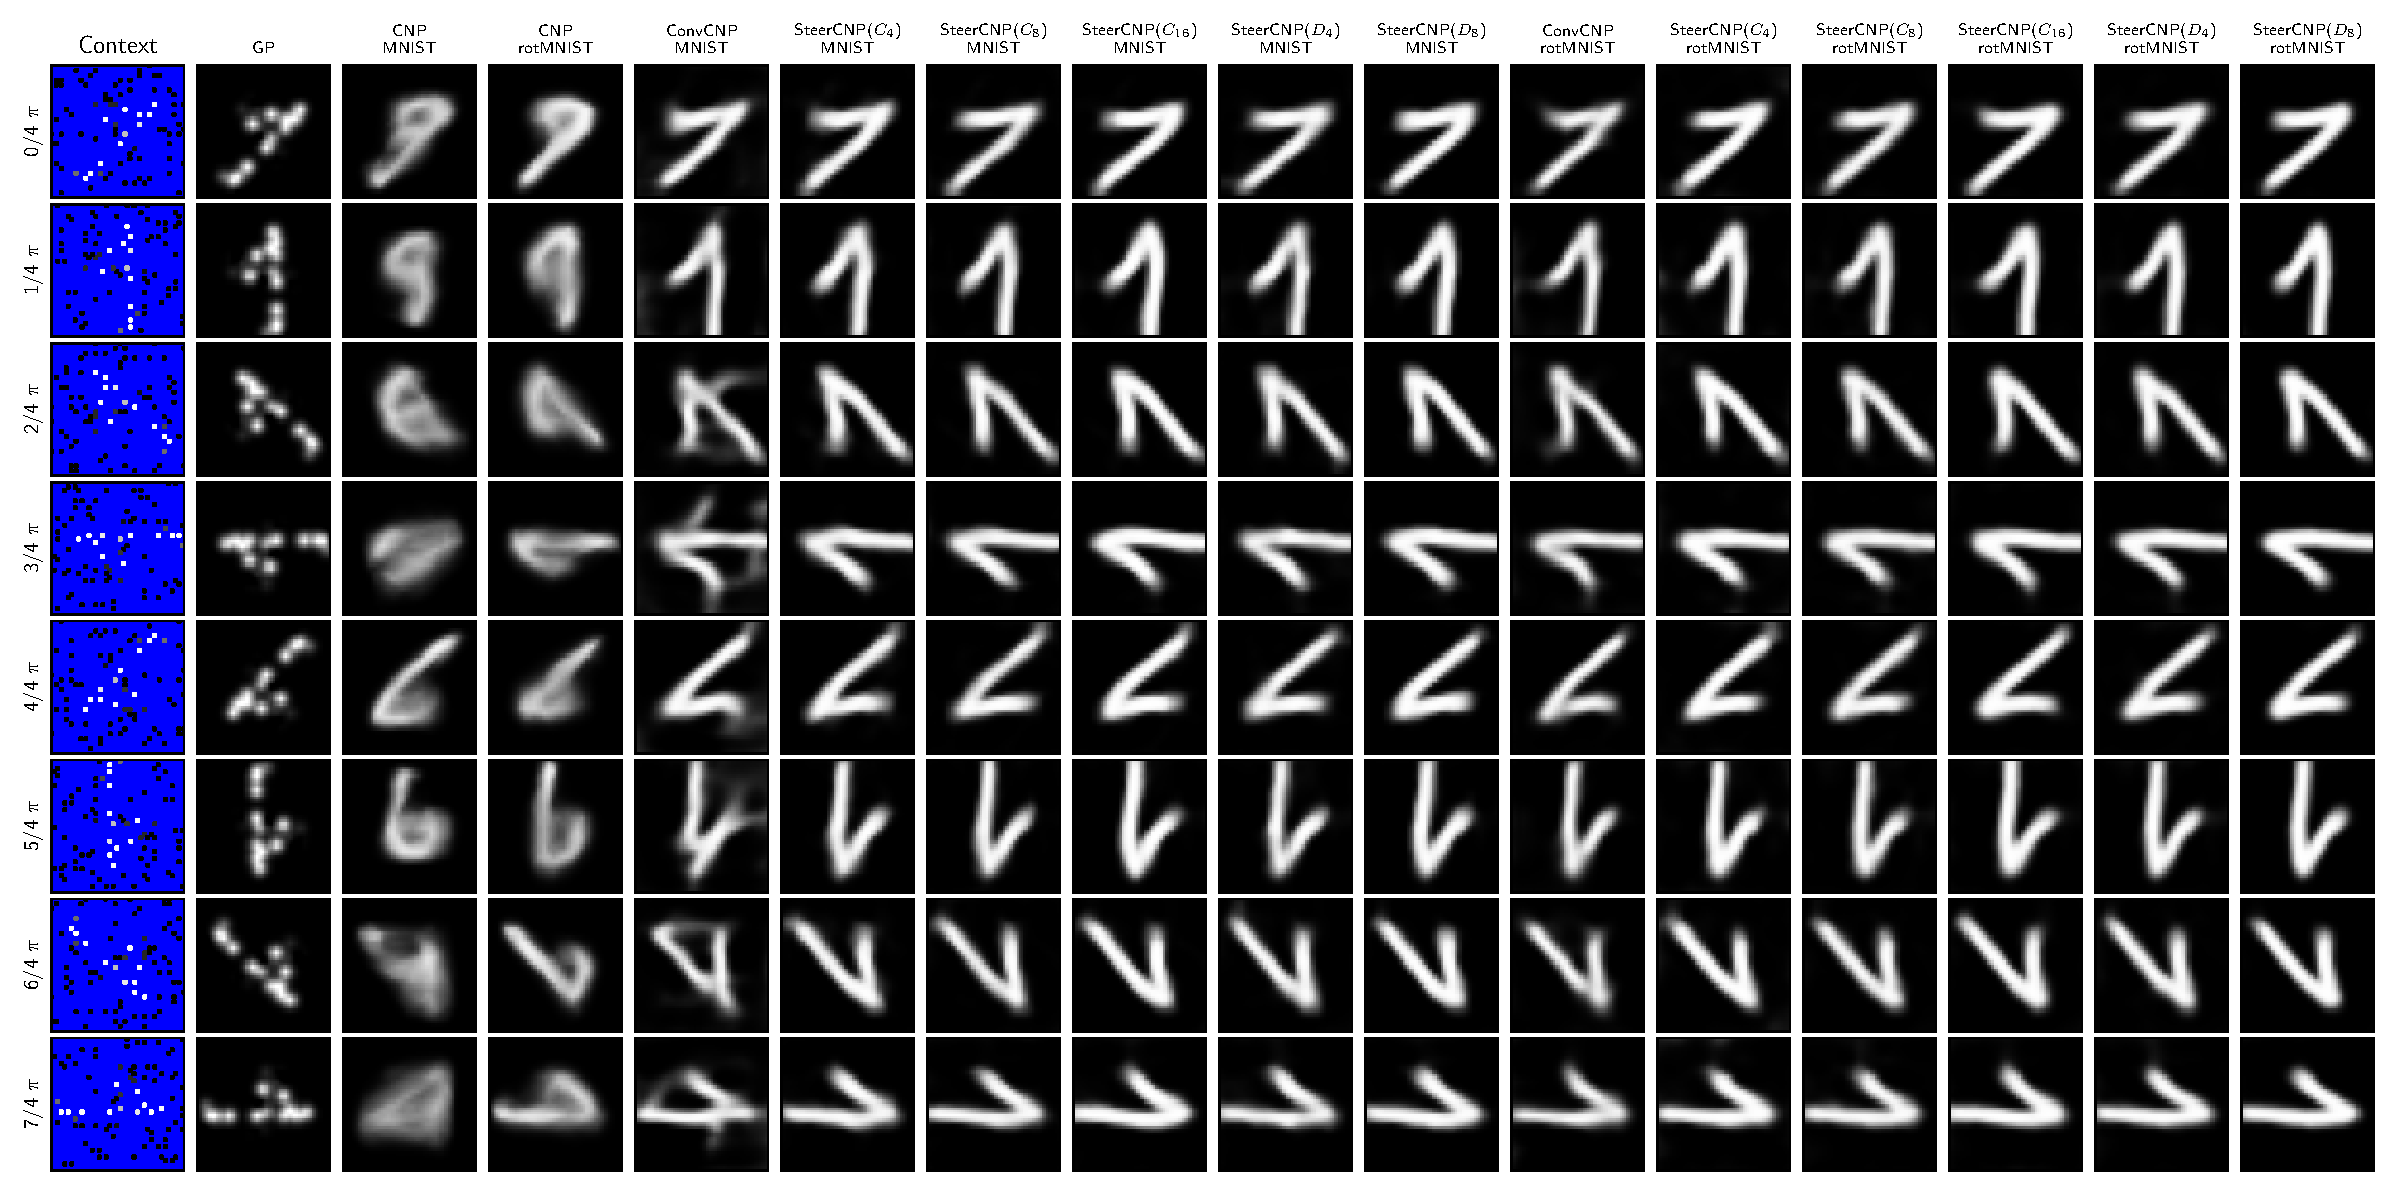
\includegraphics[width=\textwidth]{images/steer_cnps/mnist/train_rotation.pdf}
	\caption{Qualitative examples of the behaviour of the predicted mean of different models when the context set is rotated.
		We observe that the ConvCNP, even when trained on rotation augmented data, has trouble predicting good shapes when the context set is rotated.
		By comparison the equivariant models have very consistent predictions under rotation, with the $C_4$ and $D_4$ models beng exactly equivariant to $90^\circ$ rotations, and the $C_{16}$ models being exactly equivariant to $22.5^\circ$ rotations} \end{figure} 

\begin{figure}[ht] \centering 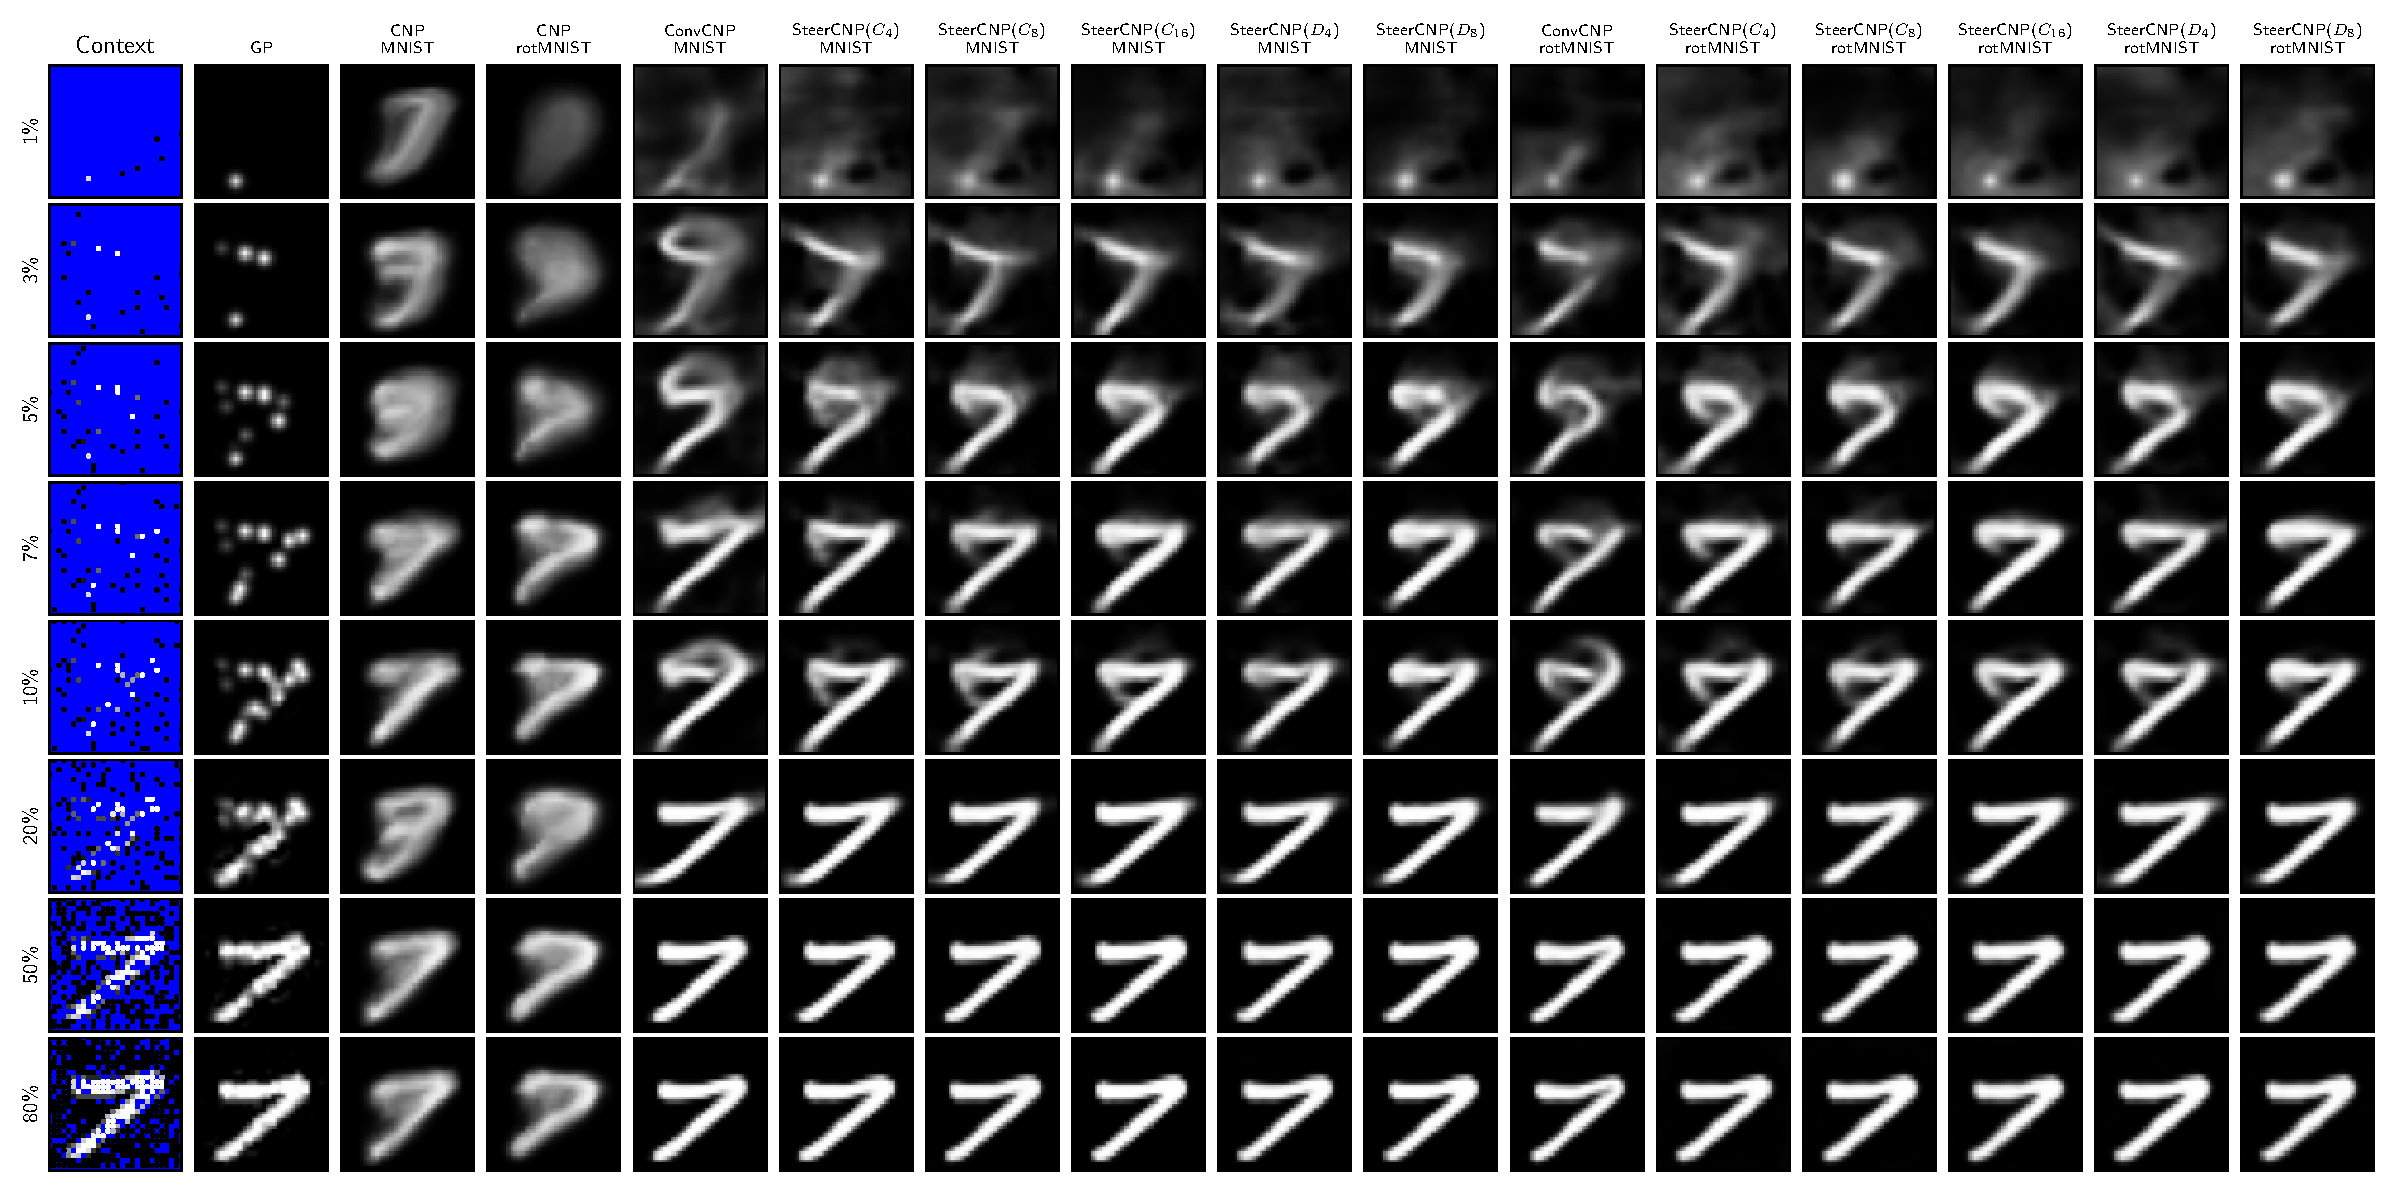
\includegraphics[width=\textwidth]{images/steer_cnps/mnist/train_percentage.pdf} \caption{Qualitative examples of the behaviour of the predicted mean of different models when the context set size is changed.
		Digit not rotated.
	}
	\centering
	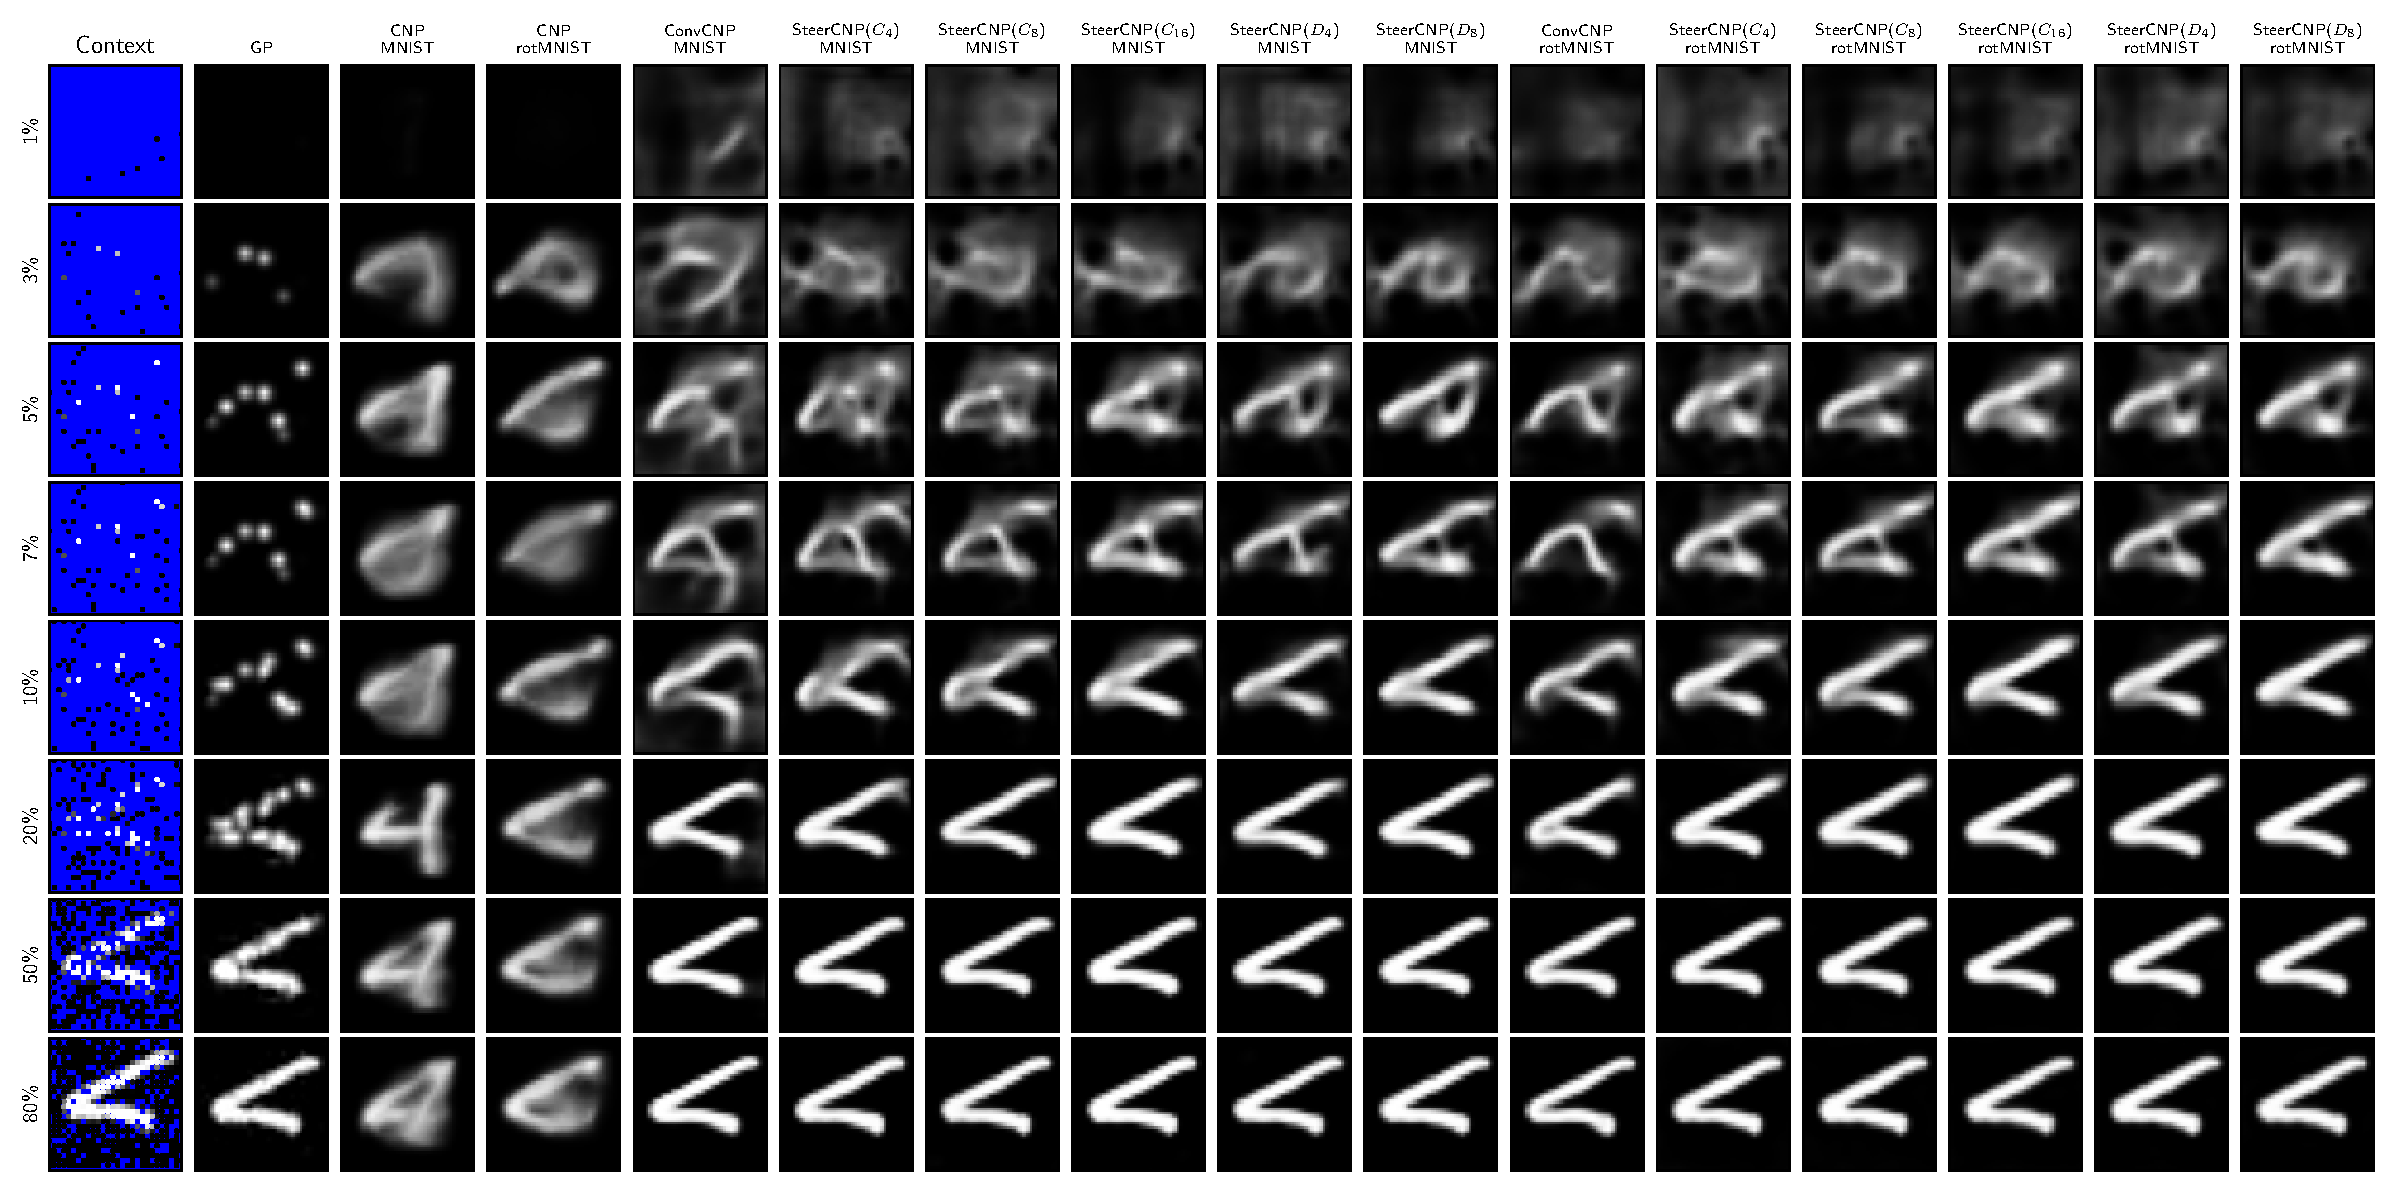
\includegraphics[width=\textwidth]{images/steer_cnps/mnist/train_rot_percentage.pdf}
	\caption{Qualitative examples of the behaviour of the predicted mean of different models when the context set size is changed.
		Digit rotated.
	}
\end{figure}

\begin{figure}[ht]
	\centering
	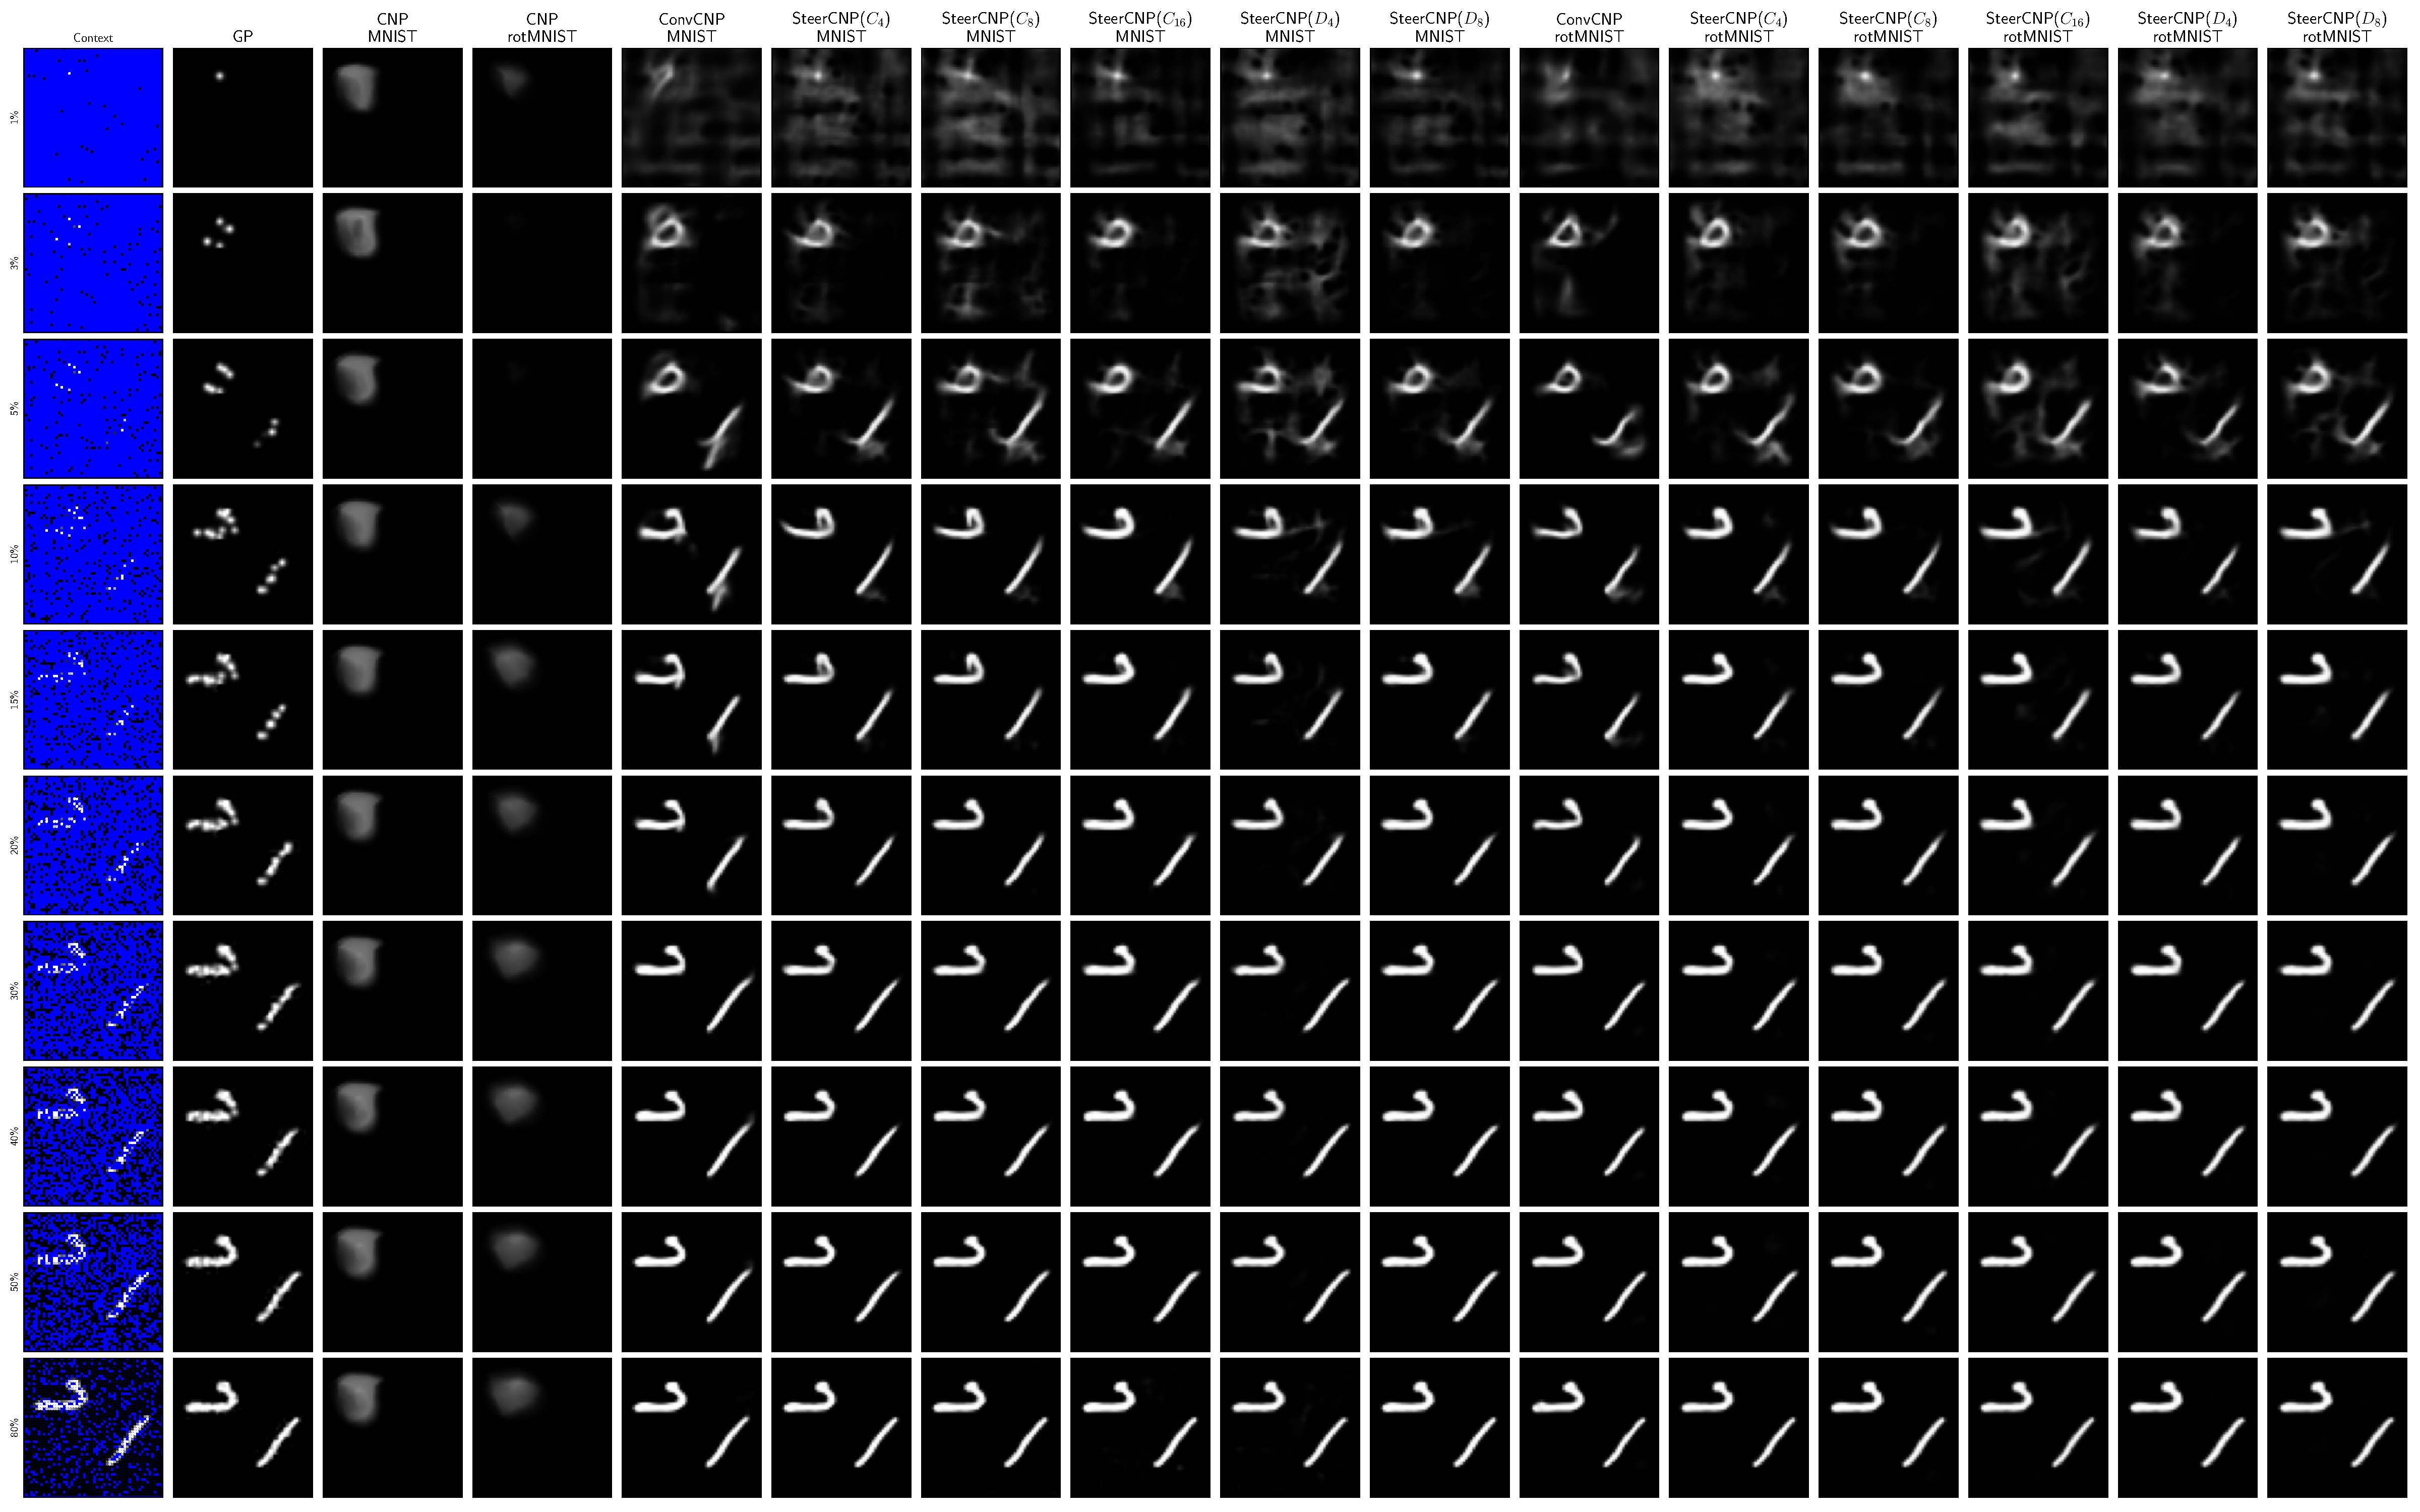
\includegraphics[width=\textwidth]{images/steer_cnps/mnist/extrapolation_percantage.pdf}
	\caption{Qualitative examples of the behaviour of models trained on single MNIST digits, tested on multiple digits pasted into a larger canvas.
		Size of context set varied.
		We see that further away from the digits there is some noise predictions.
		These are likely causes by the models never having seen data as far from digits as this, leading to somewhat undefined behaviour.
		We see that the equivariant models exhibit considerably less of this noisy behaviour.
	}
\end{figure}

\begin{figure}
	\centering
	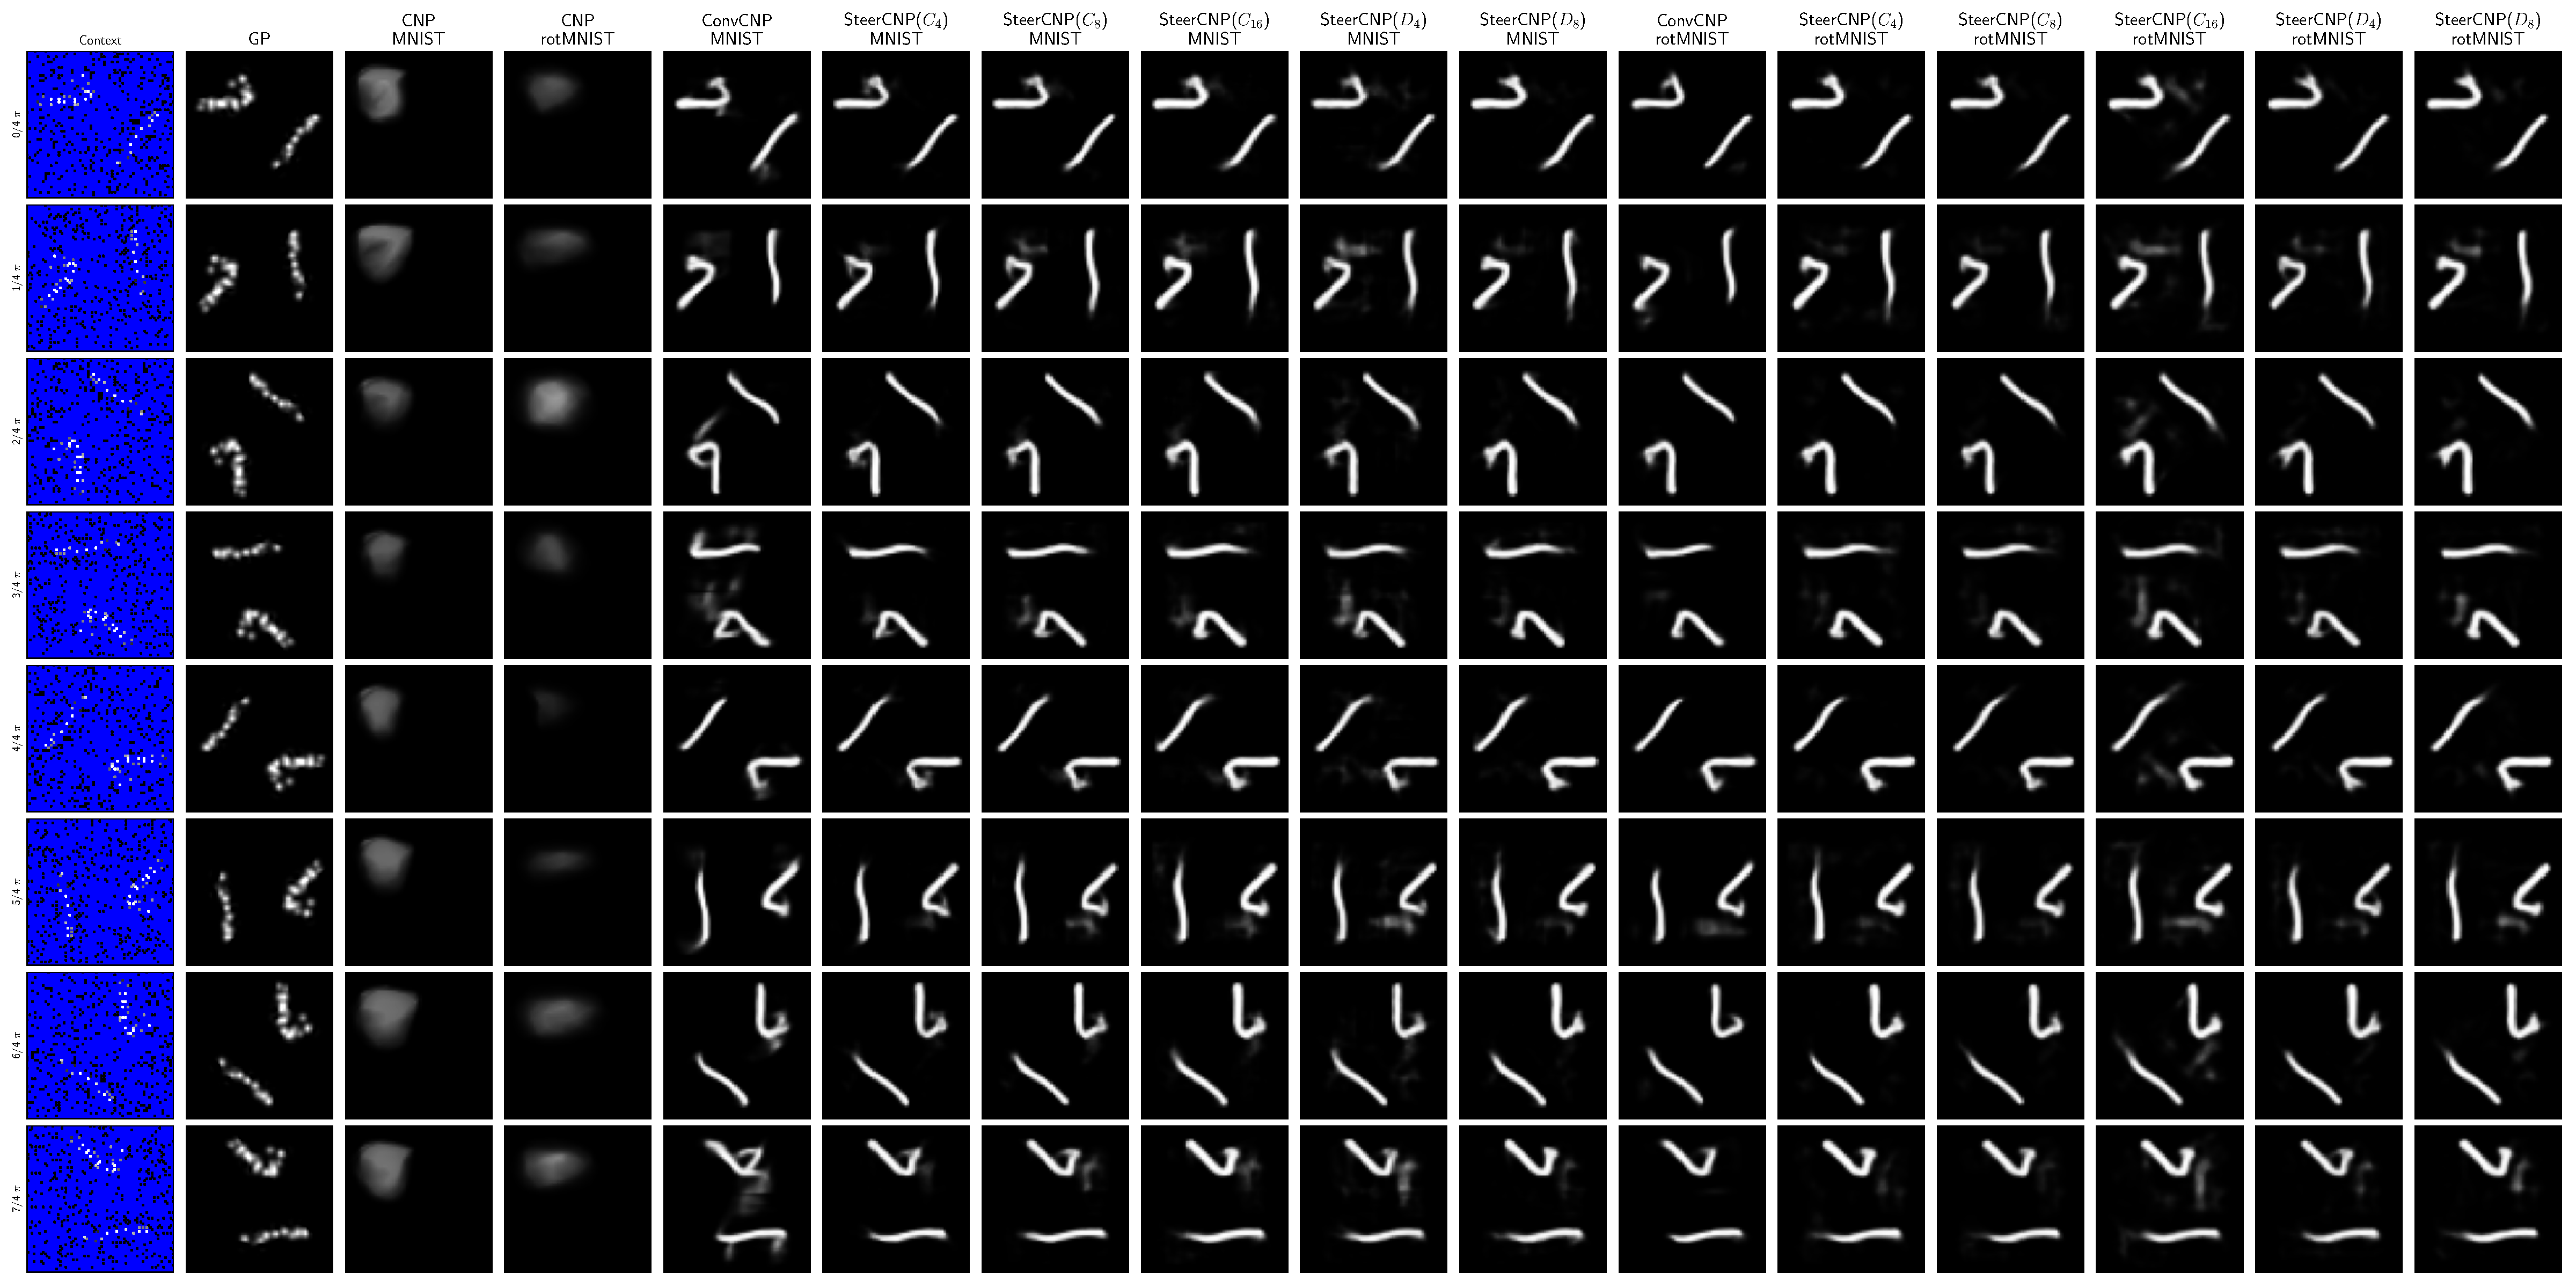
\includegraphics[width=\textwidth]{images/steer_cnps/mnist/extrapolation_rotation.pdf}
	\caption{Qualitative examples of the behaviour of models trained on single MNIST digits, tested on multiple digits pasted into a larger canvas.
		Rotation of the context set is varied.
		We see that the equivariant models show very little change in behaviour under rotation, whereas the ConvCNP gives reasonably wild predictions under rotation.
	}
\end{figure}